\documentclass[a4paper,12pt]{article}
\usepackage{geometry}
 \geometry{
 a4paper,
 total={170mm,257mm},
 left=20mm,
 top=20mm,
 }
\usepackage{adjustbox}
\usepackage[polish]{babel}
\usepackage{polski}
\usepackage{multirow}
\usepackage{makecell}
\usepackage{boldline}
\usepackage[T1]{fontenc} 
\usepackage{listings}
\usepackage{color}
\usepackage{biblatex}
\usepackage{csquotes}
\usepackage{indentfirst}
\usepackage{subfig}
\addbibresource{git.bib}

\title{Sprawozdanie z Zadania: Git}
\author{Jakub Kraus}
\date{21.01.2024}
\renewcommand\theadalign{tl}
\begin{document}
\renewcommand{\arraystretch}{2}
\begin{table}[ht]
    \centering
    \begin{adjustbox}{width=1\textwidth,center=\textwidth}
        \begin{tabular}{V{4}lV{4}c|c|c|c|c|c V{4}}
            \hlineB{4}
            \multicolumn{2}{V{4}lV{4}}{}                                         & \multicolumn{5}{lV{4}}{\textbf{Wydział Nauk Ścisłych i Technicznych}}                                                                                                                                   \\
            \cline{3-7}
            \multicolumn{2}{V{4}cV{4}}{\textbf{Uniwersytet Śląski w Katowicach}} & \multicolumn{5}{lV{4}}{\textbf{Instytut Fizyki}}                                                                                                                                                        \\
            \cline{3-7}
            \multicolumn{2}{V{4}lV{4}}{}                                         & Rok                                                                   & \textbf{III}                                          & Semestr                            & \multicolumn{2}{cV{4}}{\textbf{V}} \\
            \hlineB{4}
            Kierunek                                                             & \multicolumn{6}{cV{4}}{Informatyka stosowana}                                                                                                                                                           \\
            \hline
            Przedmiot                                                            & \multicolumn{6}{cV{4}}{\textbf{SiNWO - laboratorium}}                                                                                                                                                   \\
            \hlineB{4}
            Prowadzący                                                           & \multicolumn{6}{cV{4}}{dr Wojciech Gurdziel}                                                                                                                                                            \\
            \hline
            Tytuł ćwiczenia                                                      & \multicolumn{4}{c|}{\textbf{Wprowadzenie do git}}                     &
            \multirow{2}{*}{Nr ćwiczenia}                                        & \multirow{2}{*}{\textbf{I}}                                                                                                                                                                             \\
            \cline{1-5}
            \thead{Sprawozdanie wykonał:                                                                                                                                                                                                                                                   \\ (Imię i Nazwisko)} &
            \multicolumn{4}{c|}{\textbf{Jakub Kraus}}                            &                                                                       &                                                                                                                                 \\
            \hlineB{3}
            Data wykonania ćwiczenia                                             & \textbf{09.11.2023}                                                   & \multicolumn{2}{V{4}lV{4}}{Data oddania sprawozdania} & \multicolumn{3}{cV{4}}{31.01.2024}                                      \\
            \hlineB{4}
        \end{tabular}
    \end{adjustbox}
\end{table}

\newpage

\tableofcontents
\listoffigures

\newpage

\section{Cel ćwiczenia}
Celem ćwiczenia było zapoznanie się z podstawowymi komendami systemu kontroli wersji git oraz z ich zastosowaniem w praktyce.

\section{Przebieg ćwiczenia}
Ćwiczenie składało się z dwóch części. Pierwsza część polegała na wykonaniu zadań na platformie Learn Git Branching. Druga część polegała na wykonaniu zadań w terminalu z wykorzystaniem systemu git.

\subsection{Learn Git Branching}

\begin{figure}[!ht]
    \centering
    \subfloat[Zadania głowne]{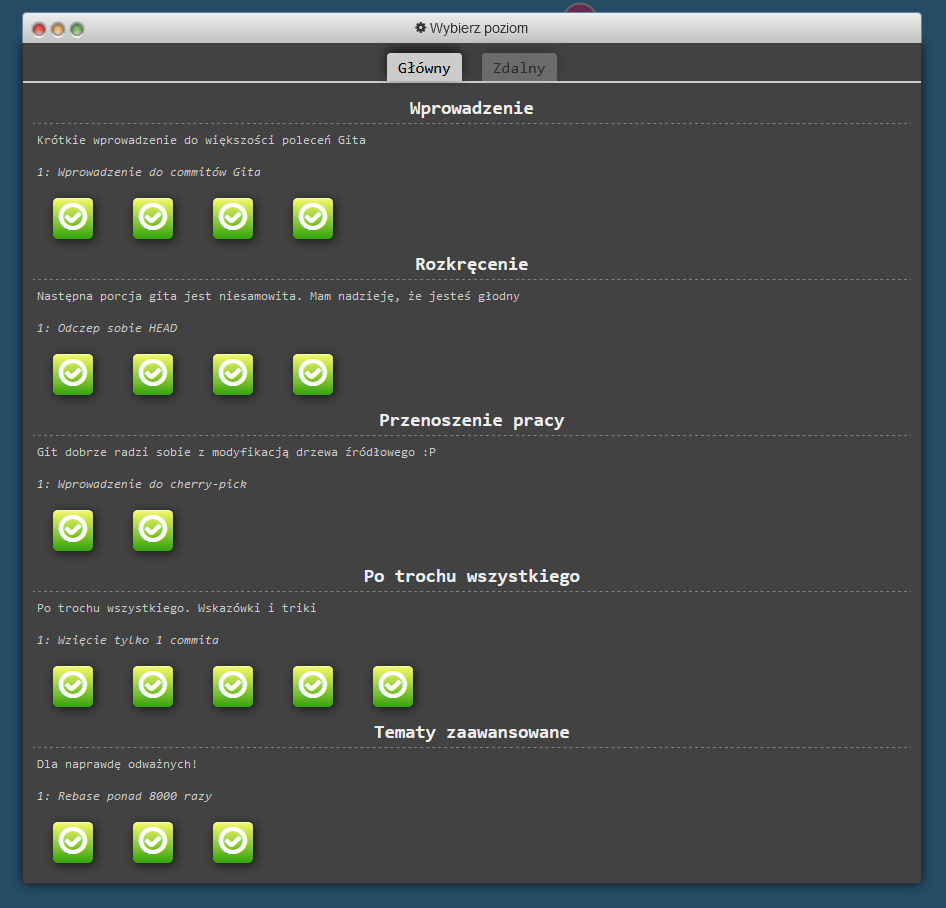
\includegraphics[width=11cm]{images/learn-git-branching.png}}
    \vfill
    \subfloat[Zadania zdalne]{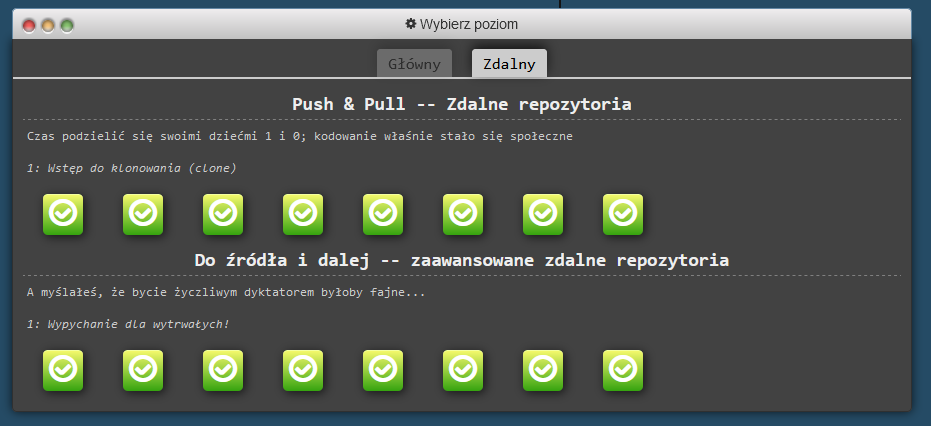
\includegraphics[width=11cm]{images/learn-git-branching-2.png}}
    \caption{Zrzuty ekranu z Learn Git Branching}
\end{figure}

\newpage

\subsection{Git}
Do wykonania ćwiczenia wykorzystałem system openSUSE Tumbleweed \cite{noauthor_opensuse_nodate} oraz serwis \\ GitHub \cite{noauthor_github:_nodate} do przechowywania repozytorium zdalnego. Wszystkie operacje wykonywałem w terminalu.
\subsubsection{Terminal}

\begin{figure}[ht]
    \centering
    \subfloat[Klonowanie oraz pierwszy commit]{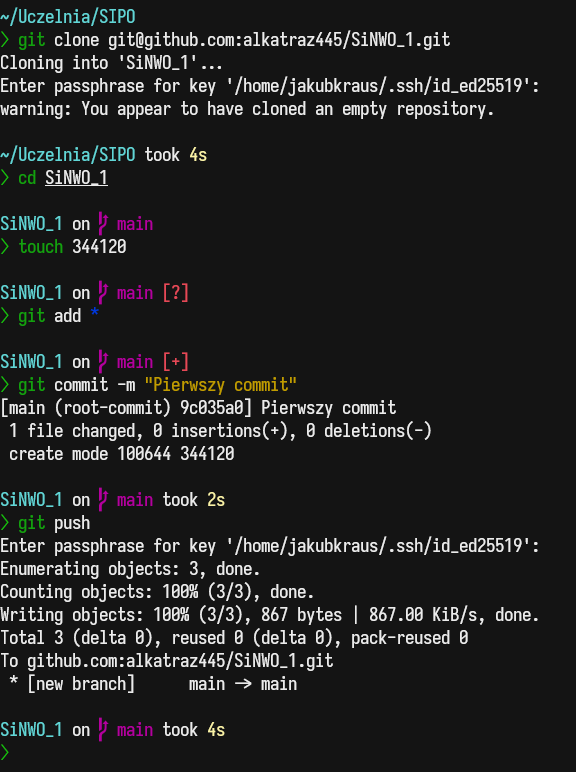
\includegraphics[width=8cm]{images/git-1.png}}
    \hfill
    \subfloat[Klonowanie do drugiego folderu]{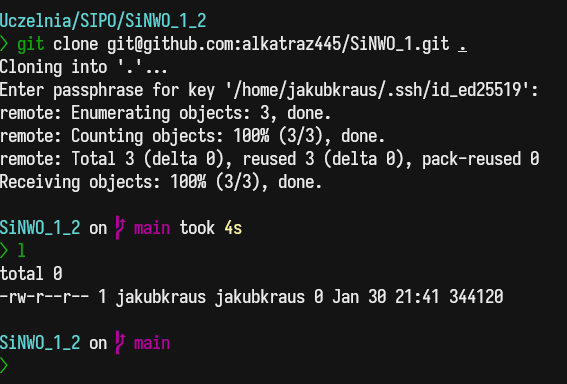
\includegraphics[width=8cm]{images/git-2.png}}
    \caption{Początek operacji na repozytorium}
\end{figure}

\begin{figure}[ht]
    \centering
    \subfloat[Dodanie zawartości pliku w pierwszym folderze oraz push do repozytorium zdalnego]{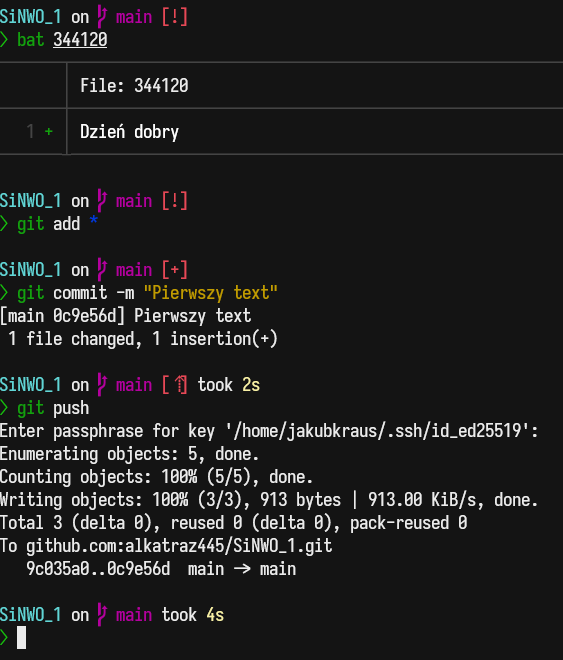
\includegraphics[width=10cm]{images/git-3.png}}
    \hfill
    \subfloat[Dodanie zawartości do pliku w drugim folderze i commit]{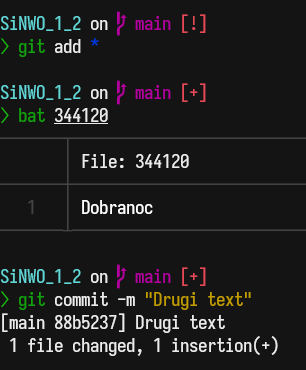
\includegraphics[width=6cm]{images/git-4.png}}
    \caption{Symulacja konfliktu danych}
\end{figure}

\newpage

\begin{figure}[ht]
    \centering
    \subfloat[Rebase]{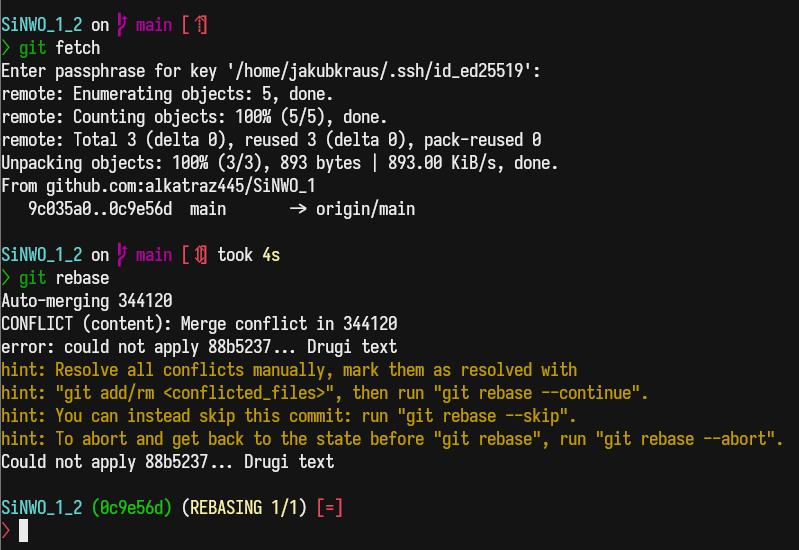
\includegraphics[width=10cm]{images/git-5.png}}
    \hfill
    \subfloat[Zaistniały konflikt]{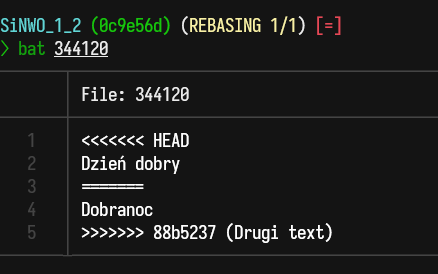
\includegraphics[width=6cm]{images/git-6.png}}
    \caption{Rebase z konfliktem}
\end{figure}

\newpage

\begin{figure}[ht]
    \centering
    \subfloat[Edycja pliku z konfliktem]{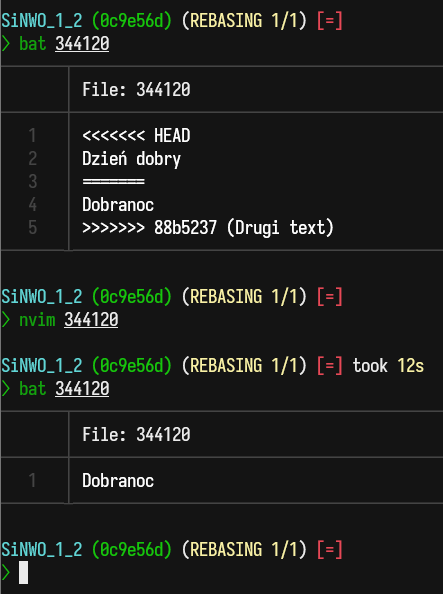
\includegraphics[width=7cm]{images/git-7.png}}
    \hfill
    \subfloat[Dokończenie rebase i pushowanie]{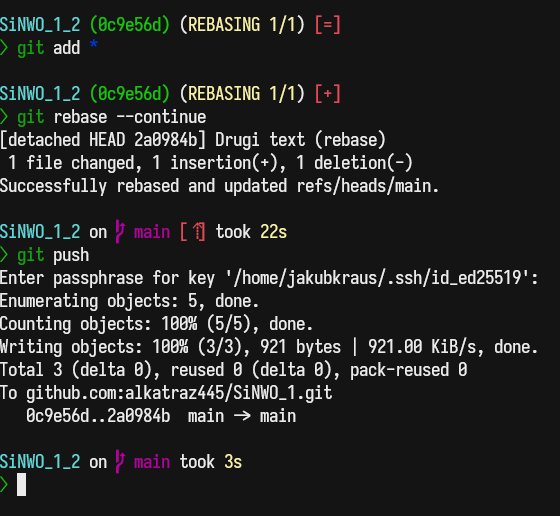
\includegraphics[width=9cm]{images/git-8.png}}
    \caption{Rozwiązanie konfliktu}
\end{figure}

\begin{figure}[hb]
    \centering
    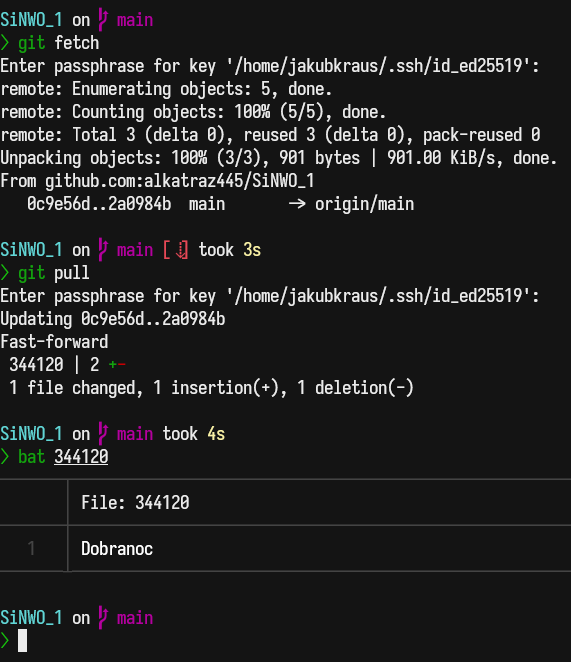
\includegraphics[width=10cm]{images/git-9.png}
    \caption{Pull z repozytorium zdalnego}
\end{figure}

\newpage
\clearpage
\begin{figure}[ht]
    \centering
    \subfloat[Tworzenie ``test\_branch'']{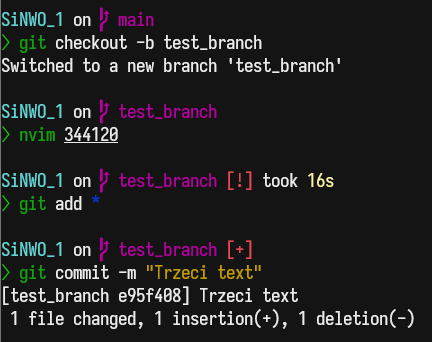
\includegraphics[width=8cm]{images/git-merge-1.png}}
    \hfill
    \subfloat[]{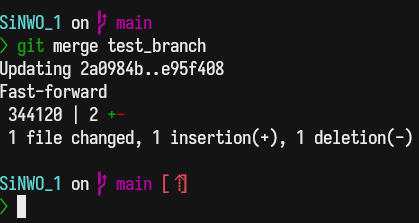
\includegraphics[width=8cm]{images/git-merge-2.png}}
    \caption{Tworzenie nowej gałęzi i przełączanie się na nią}
\end{figure}

\begin{figure}[ht]
    \centering
    \subfloat[Push do repozytorium]{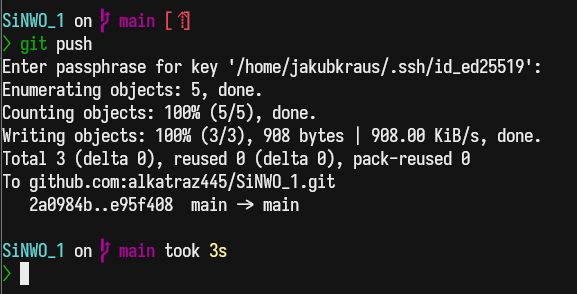
\includegraphics[width=11cm]{images/git-merge-3.png}}
    \hfill
    \subfloat[Zawartość pliku tekstowego]{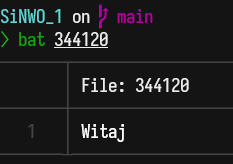
\includegraphics[width=5cm]{images/git-merge-4.png}}
    \caption{Push do repozytorium zdalnego}
\end{figure}

\clearpage

\subsubsection{Github}

\begin{figure}[ht]
    \centering
    \subfloat[Historia commitów]{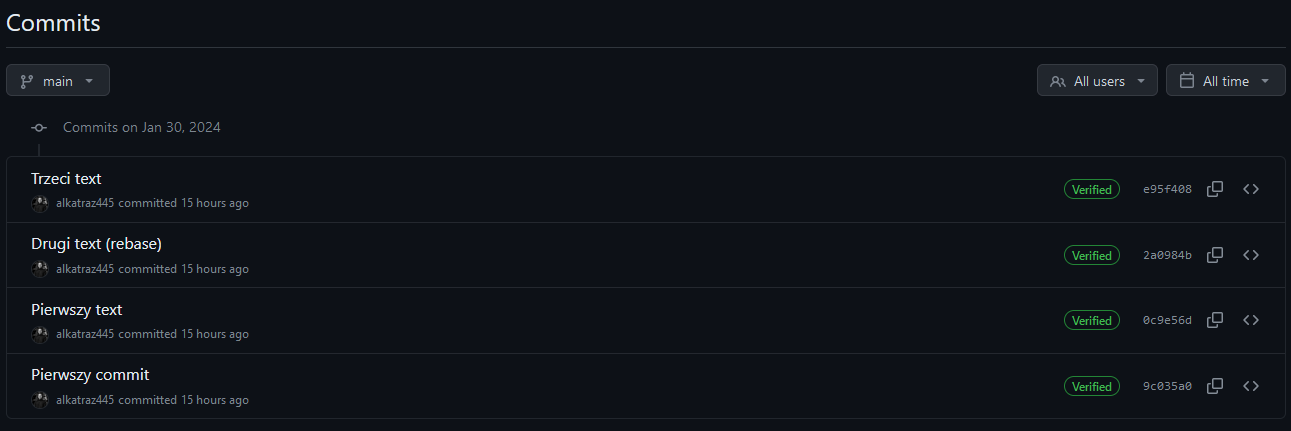
\includegraphics[width=17cm]{images/github-1.png}}
    \vfill
    \subfloat[Zawartość pliku po wszystkich zmianach]{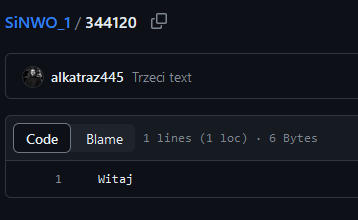
\includegraphics[width=8cm]{images/github-2.png}}
    \caption{Repozytorium na Github}
\end{figure}

\newpage
\clearpage

\section{Wnioski}
\subsection{Learn Git Branching}
Platforma ta dostarcza praktycznych ćwiczeń, które pozwalają zrozumieć i utrwalić teoretyczną wiedzę związana z Gitem. To świetne narzędzie do nauki i doskonalenia umiejętności. Learn Git Branching jest dostępny w wielu językach, w tym polskim, co zwiększa dostępność dla osób nie znających języka angielskiego.

\subsection{Git}
Zdobycie umiejętności z zakresu tworzenia, zarządzania i scalania gałęzi jest kluczowe dla organizacji pracy nad projektem. Pozwala to na równoczesne rozwijanie różnych funkcji czy poprawek bez wpływania na główną gałąź. Dzięki temu można w łatwy sposób wypróbować nowe funkcjonalności, a następnie zdecydować czy dodać je do głównej gałęzi. W przypadku konfliktu, który może wystąpić podczas scalania gałęzi, Git pozwala na wygodne rozwiązanie tego problemu. Wystarczy edytować plik z konfliktem, a następnie dokończyć operację scalania. Dzięki temu nie trzeba tworzyć nowej gałęzi, a następnie kopiować zmian z jednej gałęzi do drugiej. Wszystkie operacje związane z zarządzaniem gałęziami są bardzo proste i intuicyjne.

Warto zaznaczyć, że Git jest bardzo wydajny i nie powoduje opóźnień w pracy. Operacja pushowania do zdalnych repozytoriów trwa krótko, nawet przy relatywnie dużych plikach.

\printbibliography
\nocite{*}

\end{document}